\documentclass{SGGW-thesis}

\INZYNIERSKAtrue 
\WZIMtrue

\usepackage[T1]{fontenc}
\usepackage[utf8]{inputenc}
\usepackage{polski}
\usepackage{amsmath}
\usepackage{amssymb}
\usepackage{graphicx}
\usepackage[hidelinks]{hyperref}

\author{Adam Kliś}
\album{217584} 
\title{Projekt systemu autoryzacji w oparciu o funkcjonalność tokenów}
\Etitle{Design of an authorization system based on token functionality} 
\course{Informatyka}
\promotor{dr inż. Artur Krupa}
\pworkplace{Katedra Informatyki / Instytut Informatyki Technicznej} 
\date{Warszawa, 2026}

\geometry{
 a4paper,
 total={170mm,257mm},
 left=20mm,
 top=20mm,
}

\begin{document}
\maketitle

\section*{Słownik pojęć}
\addcontentsline{toc}{section}{Słownik pojęć}
\begin{itemize}
    \item \textbf{Autoryzacja} – proces weryfikacji, czy dany (już uwierzytelniony) użytkownik posiada uprawnienia do wykonania określonej operacji.
    \item \textbf{Uwierzytelnianie (Authentication)} – proces weryfikacji tożsamości użytkownika (np. na podstawie loginu i hasła).
    \item \textbf{Token} – cyfrowy nośnik informacji, często zabezpieczony kryptograficznie, reprezentujący tożsamość lub uprawnienia użytkownika.
    \item \textbf{API (Application Programming Interface)} – interfejs programistyczny aplikacji pozwalający na komunikację między systemami.
    \item \textbf{Zero Trust} – model bezpieczeństwa zakładający, że żadne urządzenie ani użytkownik nie jest domyślnie zaufany, nawet jeśli znajduje się wewnątrz sieci korporacyjnej.
\end{itemize}

\clearpage
\tableofcontents
\clearpage

\section{Wstęp}

Wraz z dynamicznym rozwojem aplikacji internetowych oraz popularyzacją architektury rozproszonej, mechanizmy uwierzytelniania i autoryzacji stały się jednym z najbardziej krytycznych elementów systemów informatycznych. Zapewnienie bezpieczeństwa danych, przy jednoczesnym zachowaniu wysokiej wydajności i skalowalności, stanowi wyzwanie, z którym inżynierowie oprogramowania mierzą się od początków istnienia sieci WWW. We wczesnych fazach rozwoju aplikacji internetowych serwery generowały statyczne strony HTML, a potrzeba śledzenia tożsamości użytkownika była marginalna. Z czasem standardem stało się podejście oparte na sesjach, gdzie serwer tworzył w pamięci operacyjnej obiekt sesji, a do przeglądarki klienta wysyłał jedynie identyfikator zapisywany w pliku cookie. Choć bezpieczne, rozwiązanie to utrudniało skalowanie poziome w nowoczesnych architekturach mikroserwisowych.

Współczesne podejście do cyberbezpieczeństwa coraz częściej opiera się na paradygmacie \textit{Zero Trust} (architekturze zerowego zaufania). Koncepcja ta zrywa z tradycyjnym modelem "zaufanej sieci wewnętrznej". W modelu Zero Trust zakłada się, że zagrożenie może pojawić się zewsząd, dlatego każde, nawet wewnętrzne żądanie dostępu do zasobów musi zostać rygorystycznie zweryfikowane. Oznacza to, że uwierzytelnienie przy wejściu do systemu nie jest wystarczające – niezbędna jest ciągła weryfikacja uprawnień (autoryzacja) przy każdym pojedynczym zapytaniu. Aby realizować ten postulat wydajnie, branża oprogramowania odeszła od obciążających serwery sesji na rzecz lekkich, kryptograficznie podpisanych poświadczeń.

Głównym celem niniejszej pracy inżynierskiej jest zaprojektowanie oraz implementacja autorskiego, wysoce zoptymalizowanego systemu autoryzacji w środowisku .NET, opartego o funkcjonalność tokenów. Stworzone rozwiązanie stanowi alternatywę dla standardu JWT, optymalizując narzut sieciowy oraz proces walidacji ról za pomocą operacji bitowych. Praca została podzielona na logiczne etapy, prowadząc czytelnika od przeglądu teorii i stosu technologicznego (Rozdział 2), poprzez projekt architektury i diagramy pozbawione szczegółów implementacyjnych (Rozdział 3), aż po konkretną realizację programistyczną (Rozdział 4). Dopełnieniem procesu inżynierskiego jest testowanie rozwiązania i analiza jego bezpieczeństwa w kontekście standardów branżowych, takich jak OWASP Top 10 (Rozdział 5), co ostatecznie prowadzi do podsumowania uzyskanych wyników.

\clearpage

\section{Przegląd technologii i stan wiedzy}

Aby w pełni zrozumieć architekturę proponowanego rozwiązania, konieczne jest omówienie fundamentów teoretycznych oraz technologii wykorzystywanych w nowoczesnych aplikacjach webowych. Rozdział ten wprowadza pojęcia protokołu HTTP, dogłębnie analizuje ewolucję mechanizmów utrzymania stanu, poddaje krytyce popularny standard JWT oraz definiuje stos technologiczny wybrany do implementacji autorskiego systemu.

\subsection{Uwierzytelnianie a autoryzacja}

W inżynierii bezpieczeństwa oprogramowania pojęcia uwierzytelniania i autoryzacji są często używane zamiennie, co stanowi poważny błąd terminologiczny. Zrozumienie różnicy między nimi jest kluczowe dla poprawnego modelowania systemów dostępu.

\textbf{Uwierzytelnianie (ang. Authentication - AuthN)} to proces weryfikacji tożsamości użytkownika lub systemu. Odpowiada na pytanie: "Kim jesteś?". W tradycyjnych systemach proces ten realizowany jest najczęściej poprzez podanie loginu i hasła. W rozwiązaniach bardziej zaawansowanych stosuje się biometrię lub uwierzytelnianie wieloskładnikowe (MFA).

\textbf{Autoryzacja (ang. Authorization - AuthZ)} to proces decyzyjny następujący zawsze po udanym uwierzytelnieniu. Odpowiada na pytanie: "Czy masz prawo to zrobić?". Nawet jeśli tożsamość użytkownika została poprawnie zweryfikowana, system autoryzacyjny musi sprawdzić, czy jego rola uprawnia go do dostępu do konkretnego zasobu (np. usunięcia rekordu z bazy danych). Niniejsza praca skupia się na optymalizacji obu tych procesów, ze szczególnym naciskiem na minimalizację kosztów obliczeniowych podczas ciągłej autoryzacji zapytań sieciowych.

\subsection{Protokół HTTP i problem braku stanu}

Protokół HTTP (ang. \textit{Hypertext Transfer Protocol}), będący fundamentem komunikacji w sieci Web, z definicji jest protokołem bezstanowym (ang. \textit{Stateless}). Oznacza to, że każde żądanie wysyłane przez klienta do serwera traktowane jest jako całkowicie niezależna operacja. Serwer na poziomie sieciowym nie przechowuje żadnych informacji o poprzednich interakcjach z danym klientem.

Z inżynierskiego punktu widzenia bezstanowość HTTP jest jego ogromną zaletą. Pozwala ona na szybkie obsługiwanie tysięcy jednoczesnych połączeń bez drastycznego przyrostu zużycia pamięci operacyjnej (RAM) serwera. Wymusza to jednak na twórcach oprogramowania aplikacyjnego budowę mechanizmów, które do każdego żądania dołączą dowód tożsamości użytkownika.

\subsection{Ewolucja: Od sesji stanowych do bezstanowych tokenów}

Początkowo standardem utrzymywania ciągłości pracy użytkownika było podejście oparte na sesjach (ang. \textit{Session-based Authentication}). W tym modelu serwer, po zweryfikowaniu hasła, alokował w swojej pamięci operacyjnej obiekt sesji, a klientowi odsyłał jedynie krótki identyfikator (tzw. \textit{Session ID}) za pomocą mechanizmu ciasteczek (ang. \textit{Cookies}). Przeglądarka automatycznie dołączała ten identyfikator do kolejnych zapytań, a serwer za każdym razem musiał przeszukiwać swoją pamięć lub bazę danych, aby upewnić się, że sesja jest nadal ważna.

Złotą erę tego podejścia zakończył rozwój architektury rozproszonej i chmury obliczeniowej. W środowiskach mikroserwisowych, gdzie ruch rozkładany jest na wiele niezależnych instancji serwerowych (skalowanie poziome), stanowe sesje stały się tzw. wąskim gardłem (ang. \textit{bottleneck}). Jeśli pierwsze żądanie użytkownika trafiło na serwer A, który zapisał sesję, a kolejne na serwer B, uwierzytelnienie kończyło się błędem.

Rozwiązaniem tego problemu stały się tokeny. W modelu \textit{Token-based Authentication} serwer podpisuje pakiet informacji reprezentujący tożsamość użytkownika, a następnie odsyła go do klienta. Klient przechowuje token i dołącza go do kolejnych żądań HTTP (najczęściej w nagłówku \texttt{Authorization}). Różnice w przepływie sterowania obu mechanizmów zobrazowano na Rysunku \ref{fig:session_vs_token}.

\begin{figure}[htbp]
    \centering
    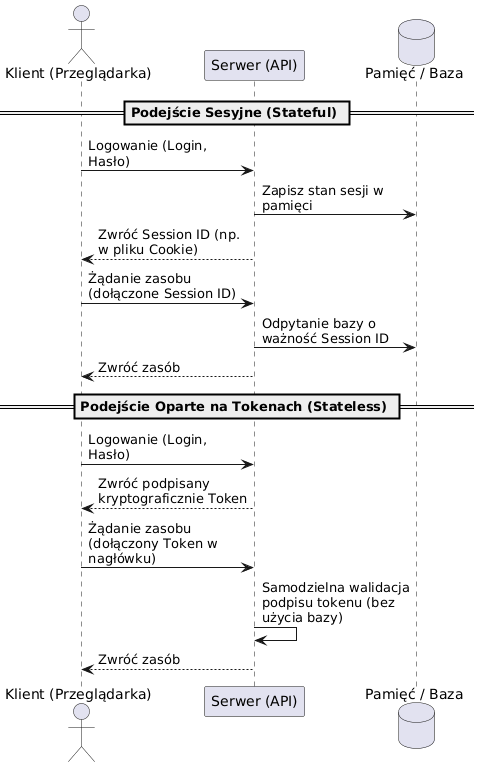
\includegraphics[width=0.8\textwidth]{png/session_vs_token.png}
    \caption{Porównanie architektury stanowej (sesyjnej) z bezstanową (tokenową)}
    \label{fig:session_vs_token}
\end{figure}

Jak widać na schemacie, podejście oparte na tokenach całkowicie odciąża bazę danych z procesu ciągłej autoryzacji – serwer samodzielnie weryfikuje podpis matematyczny.

\clearpage

\subsection{Anatomia standardu JSON Web Token (JWT)}

Najpopularniejszym rynkowym formatem tokenu jest standard JWT (zdefiniowany w dokumencie RFC 7519). Klasyczny token JWT to długi ciąg znaków (często przekraczający 500 bajtów), który składa się z trzech części oddzielonych kropkami:

\textbf{1. Nagłówek (Header):} Definiuje typ tokenu oraz algorytm kryptograficzny użyty do podpisu. Zazwyczaj ma postać prostego obiektu JSON:
\begin{verbatim}
{
  "alg": "HS256",
  "typ": "JWT"
}
\end{verbatim}

\textbf{2. Ładunek (Payload):} Miejsce przechowywania oświadczeń (ang. \textit{claims}), czyli faktycznych danych o użytkowniku, takich jak jego identyfikator (\texttt{sub}), data wygaśnięcia (\texttt{exp}) czy posiadane uprawnienia. W standardzie JWT role przesyłane są zazwyczaj jako pełne ciągi tekstowe:
\begin{verbatim}
{
  "sub": "1234567890",
  "name": "Jan Kowalski",
  "roles": ["admin", "moderator", "user"],
  "exp": 1516239022
}
\end{verbatim}

\textbf{3. Podpis (Signature):} Kryptograficzny skrót obliczony z zakodowanego nagłówka i ładunku przy użyciu klucza tajnego.

Krytyczna analiza tego standardu uwidacznia jego redundancję w zamkniętych środowiskach mikroserwisowych. Przesyłanie w każdym pojedynczym żądaniu nagłówka informującego o typie algorytmu jest zbędnym narzutem danych, ponieważ aplikacja odczytująca token posiada już tę wiedzę z własnej konfiguracji wewnętrznej. Ponadto, tekstowy zapis ról potęguje objętość ładunku. Wyeliminowanie tych nadmiarowych elementów stało się główną motywacją do stworzenia autorskiego formatu opisanego w niniejszej pracy.

\subsection{Paradygmat Inversion of Control i mechanizm DI}

Zastosowany stos technologiczny wymusza na programistach przestrzeganie dobrych praktyk projektowych. Jednym z najważniejszych paradygmatów zastosowanych w architekturze biblioteki jest odwrócenie sterowania (ang. \textit{Inversion of Control} -- IoC) realizowane poprzez wzorzec Wstrzykiwania Zależności (ang. \textit{Dependency Injection} -- DI). 

Zasada ta jest bezpośrednio powiązana z literą "D" w akronimie SOLID (ang. \textit{Dependency Inversion Principle}), która mówi, że moduły wysokopoziomowe nie powinny zależeć od modułów niskopoziomowych, a obie warstwy powinny opierać się na abstrakcjach. Zamiast bezpośrednio tworzyć instancje obiektów (np. połączeń do bazy danych) wewnątrz klas przy użyciu słowa kluczowego \texttt{new}, komponenty systemu deklarują swoje zależności poprzez interfejsy w konstruktorach.

W ekosystemie ASP.NET Core wbudowany kontener DI samodzielnie zarządza cyklem życia obiektów. Rozwiązanie to jest krytyczne dla autorskiego systemu autoryzacji, ponieważ zapewnia mu wymaganą hermetyzację, wysoką testowalność (łatwe wstrzykiwanie atrap – tzw. mocków) oraz modułowość pozwalającą na integrację z dowolnym środowiskiem sieciowym.

\subsection{Środowisko uruchomieniowe i persystencja danych}

Do realizacji projektu wybrano środowisko uruchomieniowe \textbf{.NET} oraz język \textbf{C\#}. Platforma ta, rozwijana przez firmę Microsoft, stanowi obecnie jeden z najbardziej zaawansowanych i wydajnych ekosystemów do budowy wielowątkowych aplikacji serwerowych (Web API).

Istotnym elementem architektury jest warstwa persystencji danych. Interakcja z relacyjną bazą danych odbywa się za pośrednictwem technologii Entity Framework Core (EF Core). Jest to zaawansowane narzędzie klasy ORM (ang. \textit{Object-Relational Mapping}), które rozwiązuje problem tzw. niedopasowania impedancji (ang. \textit{impedance mismatch}) pomiędzy światem programowania obiektowego a tabelami bazy danych.

Wykorzystanie EF Core pozwala na operowanie na bazie bez konieczności pisania jawnych zapytań w języku SQL. Kodowanie odbywa się przy pomocy składni LINQ (ang. \textit{Language Integrated Query}), a framework automatycznie tłumaczy te komendy na bezpieczny i zoptymalizowany pod dany silnik dialekt SQL. Użycie tego narzędzia automatycznie zabezpiecza autorski system autoryzacji przed jednym z najgroźniejszych ataków sieciowych – \textit{SQL Injection} – ponieważ wszystkie wartości wstawiane do bazy są domyślnie traktowane jako parametryzowane dane wejściowe.
\clearpage

\section{Projekt i architektura systemu}

Architektura omawianego systemu została zoptymalizowana pod kątem redukcji narzutu sieciowego oraz błyskawicznej walidacji. W tym rozdziale zaprezentowano projekt mechanizmów wewnętrznych, sformalizowane modele matematyczne algorytmów oraz przepływy procesów. Zgodnie z dobrymi praktykami dokumentacji architektonicznej, celowo pominięto na tym etapie bezpośrednie implementacje kodowe, skupiając się na logice systemowej.

\subsection{Koncepcja autorskiego tokenu}

W przeciwieństwie do powszechnych standardów, autorski token został zaprojektowany z myślą o minimalizacji przesyłanych bajtów. Jest to ciąg znaków składający się zaledwie z dwóch segmentów: ładunku ($B$) zawierającego właściwe oświadczenia i dane użytkownika oraz sumy kontrolnej ($S$). 

Proces powstawania tokenu $T$ można sformalizować za pomocą następującego równania:

$$ T = \text{Base64Url}(B) + \text{"."} + \text{Base64Url}(S) $$

gdzie:
\begin{itemize}
    \item $T$ – finalny ciąg znaków reprezentujący token autoryzacyjny, przesyłany w nagłówku zapytania HTTP.
    \item $B$ – ładunek (ang. \textit{Body/Payload}), będący tekstową reprezentacją zserializowanego obiektu JSON, przechowującego dane sesji (np. zdekodowaną maskę ról oraz czas wygaśnięcia).
    \item $S$ – suma kontrolna (ang. \textit{Signature}), będąca binarnym wynikiem operacji kryptograficznej zabezpieczającej ładunek.
    \item $\text{Base64Url}()$ – funkcja kodująca dane do bezpiecznego formatu tekstowego.
\end{itemize}

Kluczowym zabiegiem inżynieryjnym w tym równaniu jest użycie algorytmu \textbf{Base64Url} zamiast standardowego Base64. Standardowe kodowanie wprowadza znaki takie jak \texttt{+} oraz \texttt{/}, które posiadają specjalne znaczenie w adresach URL i nagłówkach HTTP (mogą prowadzić do błędów parsowania). Base64Url zastępuje je odpowiednio znakami \texttt{-} (myślnik) oraz \texttt{\_} (podkreślenie), a także usuwa znaki dopełnienia \texttt{=}, co gwarantuje pełną kompatybilność protokołu sieciowego.

\subsection{Algorytm podpisu cyfrowego}

Bezpieczeństwo systemu opiera się na zapewnieniu integralności i niezaprzeczalności emitowanych poświadczeń. Do generowania sumy kontrolnej ($S$) wykorzystano algorytm symetryczny HMAC (ang. \textit{Keyed-Hash Message Authentication Code}) w oparciu o silną funkcję skrótu SHA-256. 

Wybór kryptografii symetrycznej podyktowany jest niespotykaną wydajnością oraz specyfiką aplikacji monolitycznych, gdzie serwer wydający i weryfikujący to ten sam podmiot, posiadający bezpieczny dostęp do pamięci operacyjnej. Pełny proces generowania podpisu $\sigma$ można wyrazić wzorem matematycznym:

$$ \sigma = \text{Base64Url}(\text{HMAC}_{\text{SHA256}}(K, P)) $$

gdzie poszczególne zmienne oznaczają:
\begin{itemize}
    \item $\sigma$ – ostateczny, tekstowy podpis dołączany na końcu tokenu.
    \item $K$ – klucz tajny (ang. \textit{Secret Key}), będący ciągiem znaków o wysokiej entropii, zdefiniowanym w bezpiecznej konfiguracji środowiskowej serwera. Klucz ten nigdy nie jest przesyłany do klienta.
    \item $P$ – ładunek wejściowy, czyli zakodowana już w Base64Url część danych ($P = \text{Base64Url}(B)$).
    \item $\text{HMAC}_{\text{SHA256}}$ – kryptograficzna funkcja mieszająca, która w bezpieczny sposób łączy klucz tajny z wiadomością, odporna na ataki typu \textit{Length Extension Attack}.
\end{itemize}

Przepływ danych w procesie generowania tokenu, od momentu pobrania obiektu po uzyskanie końcowego ciągu znaków, zaprezentowano na Rysunku \ref{fig:token_crypto_flow}.

\begin{figure}[htbp]
    \centering
    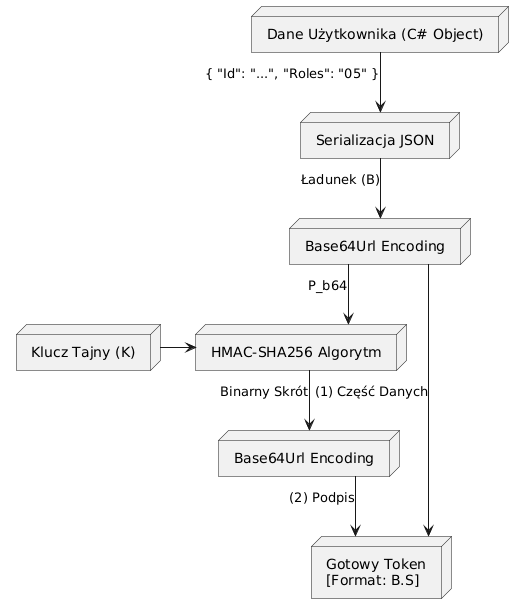
\includegraphics[width=0.75\textwidth]{png/token_crypto_flow.png}
    \caption{Architektura kryptograficzna generowania tokenu}
    \label{fig:token_crypto_flow}
\end{figure}

\subsection{Weryfikacja tokenu i integralność}

Zrozumienie procesu weryfikacji jest kluczowe z perspektywy bezpieczeństwa. Weryfikacja nie polega na kryptograficznym "odszyfrowywaniu" sumy kontrolnej, lecz na procesie jej reprodukcji.

Kiedy serwer odbiera token z żądania HTTP, rozdziela go używając znaku kropki jako separatora. Następnie, korzystając z przechwyconego ładunku $P$ oraz własnego klucza symetrycznego $K$, ponownie wykonuje funkcję $\text{HMAC}_{\text{SHA256}}$. Jeśli nowo wyliczona sygnatura $\sigma'$ jest matematycznie tożsama z sygnaturą $\sigma$ nadesłaną przez klienta ($\sigma' == \sigma$), serwer nabiera pewności, że dane nie uległy manipulacji. Ewentualna zmiana choćby jednego bitu w ładunku (np. próba zmiany identyfikatora roli) spowoduje drastyczną zmianę wyliczonego skrótu zjawiskiem lawinowym (ang. \textit{Avalanche Effect}), co poskutkuje natychmiastowym odrzuceniem żądania HTTP z kodem 401 Unauthorized.

\subsection{Zarządzanie rolami przy użyciu masek bitowych}

Największą innowacją zaprojektowanego systemu jest całkowite odejście od tekstowej reprezentacji uprawnień. Model ten opiera się na matematycznej teorii zbiorów oraz systemie wag dwójkowych.

Niech $R$ stanowi zbiór wszystkich dostępnych ról w systemie, a każda rola $r \in R$ posiada unikalny indeks liczbowy $ID_r \in \{0, 1, 2, ..., n\}$. Zbiór ról przypisanych do konkretnego użytkownika oznaczmy jako $U \subseteq R$. Maska bitowa $M$ dla danego użytkownika obliczana jest jako suma potęg liczby 2:

$$ M = \sum_{r \in U} 2^{ID_r} $$

Dla przykładu, jeżeli system posiada role "user" ($ID=0$) oraz "admin" ($ID=2$), a użytkownik posiada obie z nich, jego maska wynosi:
$$ M = 2^0 + 2^2 = 1 + 4 = 5 $$

Liczba dziesiętna 5 jest następnie konwertowana do formatu szesnastkowego (\texttt{05}) i w takiej skompresowanej formie umieszczana w ładunku tokenu.

Kiedy użytkownik żąda dostępu do zasobu zabezpieczonego konkretną rolą $r_{req}$, serwer weryfikujący nie musi przeszukiwać list ani struktur tekstowych. Wykonuje on wyłącznie jedną, natywną dla procesora operację iloczynu bitowego (AND). Dostęp zostaje przyznany wtedy i tylko wtedy, gdy spełniony jest warunek:

$$ (M \text{ AND } 2^{ID_{req}}) \neq 0 $$

Działanie to omija kosztowną alokację pamięci, czyniąc proces weryfikacji niezwykle wydajnym.

\subsection{Analiza złożoności obliczeniowej i pamięciowej}

Sformalizowanie ról do postaci masek bitowych przynosi wymierne korzyści, co można udowodnić za pomocą notacji asymptotycznej (\textit{Big O Notation}). 

W standardowym podejściu (klasyczny JWT), role weryfikowane są poprzez iteracyjne przeszukiwanie tablicy ciągów znaków. Dla $N$ ról posiadanych przez użytkownika oraz $M$ ról wymaganych przez punkt końcowy, złożoność obliczeniowa najgorszego przypadku wynosi $O(N \cdot M)$. Ponadto, operacje na łańcuchach znaków (ang. \textit{string comparisons}) dodatkowo obciążają pamięć sterty (ang. \textit{Heap}) oraz wirtualną maszynę odśmiecającą pamięć (\textit{Garbage Collector}).

W mechanizmie autorskim, po początkowym zdekodowaniu krótkiej maski szesnastkowej, proces walidacji sprowadza się do wywołania operatorów sprzętowych procesora. Złożoność obliczeniowa porównania bitowego, bez względu na wielkość słownika ról w systemie, jest stała i wynosi zawsze $\boldsymbol{O(1)}$. Złożoność pamięciowa została zredukowana do alokacji pojedynczych zmiennych typów prostych (ang. \textit{Value Types}).

\subsection{Cykl życia sesji i rotacja tokenów odświeżających}

Krótki czas życia tokenu dostępowego (zazwyczaj od kilku do kilkunastu minut) stanowi fundament bezpieczeństwa w modelu bezstanowym. Ograniczenie to drastycznie minimalizuje okno czasowe, w którym przechwycony token mógłby posłużyć do wyrządzenia szkód w systemie.

Aby zapewnić ciągłość pracy bez wymuszania na użytkowniku ciągłego wpisywania hasła, wprowadzono długoterminowe tokeny odświeżające (ang. \textit{Refresh Tokens}). Architektura zakłada wdrożenie mechanizmu rotacji (ang. \textit{Refresh Token Rotation}). 

Gdy token dostępowy traci ważność, aplikacja kliencka wysyła na dedykowany punkt końcowy token odświeżający. Jest to jedyny etap, w którym system wykonuje operację stanową (odpytuje relacyjną bazę danych). Po zweryfikowaniu kryptograficznym serwer upewnia się, że token istnieje w bazie i nie uległ przedawnieniu. Jeśli weryfikacja powiedzie się, stary token jest bezzwłocznie usuwany, a system emituje nową parę kluczy (nowy Access Token oraz nowy Refresh Token). Mechanizm ten gwarantuje, że skradziony token odświeżający będzie dla atakującego jednorazowy – gdy tylko prawowity użytkownik wygeneruje nową sesję, stary identyfikator zostanie bezpowrotnie unieważniony.

\subsection{Diagram klas: Warstwa danych}

Z uwagi na zastosowanie wzorców inżynieryjnych system podzielono na logiczne pakiety, co zilustrowano za pomocą graficznej notacji UML. Rysunek \ref{fig:class_entities} prezentuje encje bazodanowe mapujące obiekty C\# na struktury relacyjne bazy. Widoczne jest powiązanie użytkownika z odpowiednimi tokenami odświeżającymi (relacja jeden-do-wielu), oraz przypisanie uprawnień poprzez tabelę asocjacyjną \texttt{UserRole}.

\begin{figure}[htbp]
    \centering
    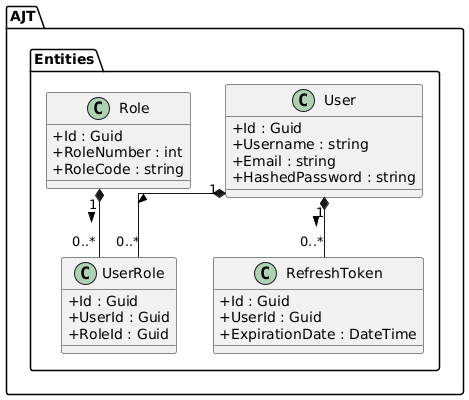
\includegraphics[width=0.7\textwidth]{png/class_entities.png}
    \caption{Diagram klas warstwy danych (Entities)}
    \label{fig:class_entities}
\end{figure}

\subsection{Diagram klas: Kontrakty i modele}

Rysunek \ref{fig:class_contracts} obrazuje obiekty transferu danych (DTO), takie jak model \texttt{Token} oraz jego zagnieżdżone elementy. Separacja abstrakcyjnych interfejsów (np. \texttt{IHashingService}) od ich implementacji fizycznych jest strukturalnym wymogiem obsługi wbudowanego kontenera Wstrzykiwania Zależności.

\begin{figure}[htbp]
    \centering
    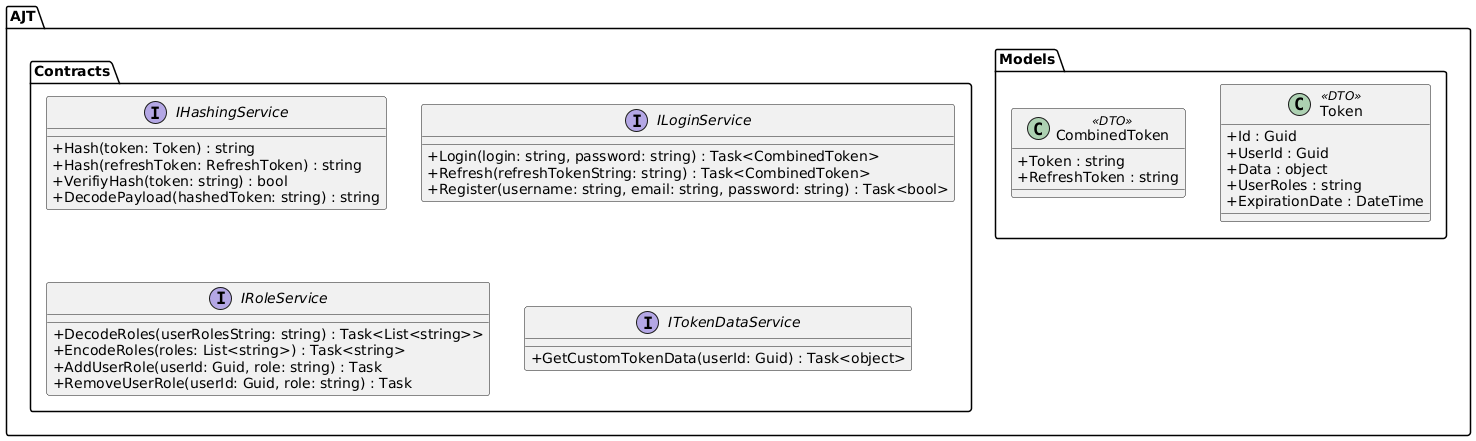
\includegraphics[width=0.8\textwidth]{png/class_contracts.png}
    \caption{Diagram klas warstwy kontraktów i modeli}
    \label{fig:class_contracts}
\end{figure}

\subsection{Diagram klas: Logika i punkty dostępu}

Ostatni schemat statyczny (Rysunek \ref{fig:class_services}) skupia się na relacjach operacyjnych w warstwie biznesowej. Obrazuje zależność między wbudowanymi filtrami autoryzacyjnymi przechwytującymi żądania HTTP, a wstrzykiwanymi do nich implementacjami serwisów przetwarzającymi maski bitowe.

\begin{figure}[htbp]
    \centering
    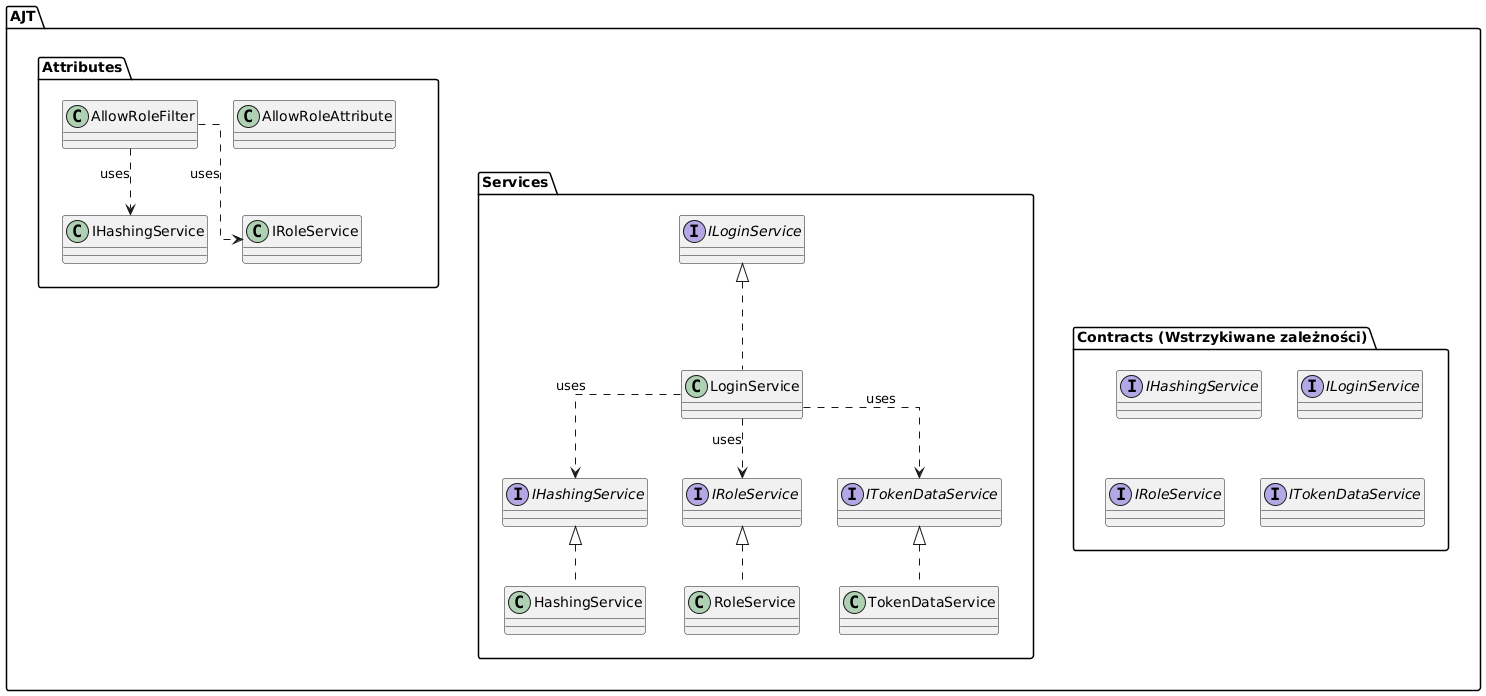
\includegraphics[width=0.85\textwidth]{png/class_services.png}
    \caption{Diagram klas implementacji logiki biznesowej}
    \label{fig:class_services}
\end{figure}

\clearpage

\subsection{Diagram przypadków użycia}

Zidentyfikowano trzech głównych aktorów wchodzących w interakcję z modułem (gość, użytkownik zalogowany, administrator). Jak zobrazowano na Rysunku \ref{fig:usecase_diagram}, architektura opiera się na dziedziczeniu uprawnień, gdzie wyższy poziom dostępu wchłania kompetencje poziomu niższego, odblokowując zarazem administracyjne punkty dostępowe.

\begin{figure}[htbp]
    \centering
    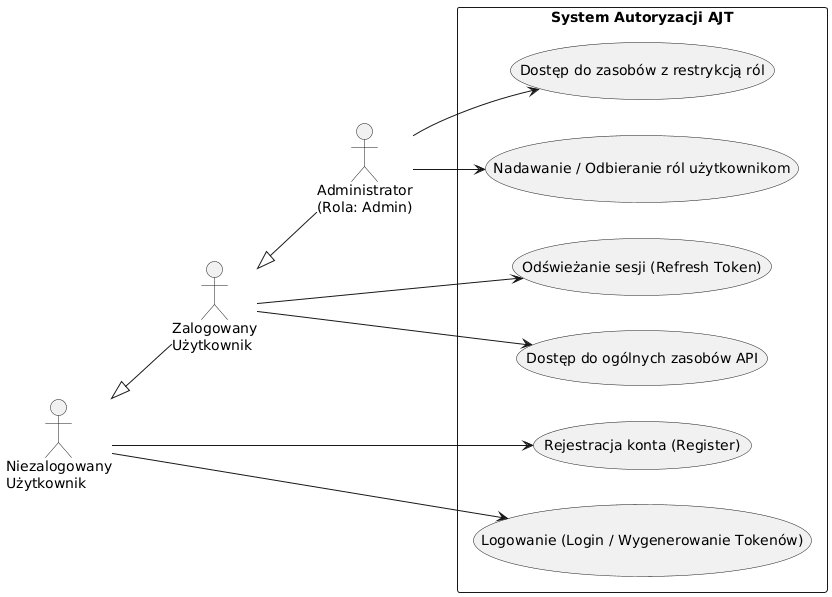
\includegraphics[width=0.8\textwidth]{png/usecase_diagram.png}
    \caption{Diagram przypadków użycia systemu}
    \label{fig:usecase_diagram}
\end{figure}

\subsection{Diagram sekwencji weryfikacji uprawnień}

Sekwencyjny przepływ weryfikacji dostępu przedstawiono na Rysunku \ref{fig:sequence_diagram}. Proces ten aktywuje się w momencie dotarcia żądania HTTP do serwera, tuż przed wywołaniem właściwej logiki domenowej. Przedstawiono w nim cykl życia walidacji: od weryfikacji kryptograficznej, przez dekodowanie matematycznej maski ról, aż po ostateczne przerwanie lub kontynuację potoku wykonawczego.

\begin{figure}[htbp]
    \centering
    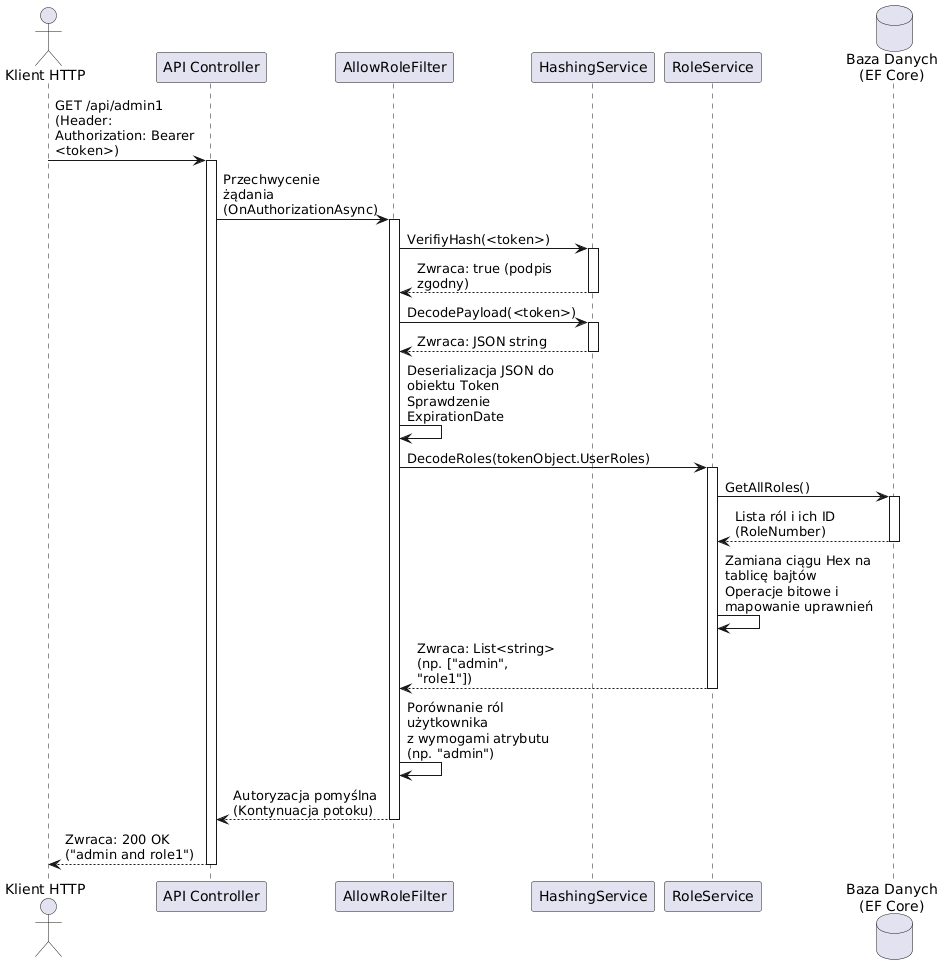
\includegraphics[width=1\textwidth]{png/sequence_diagram.png}
    \caption{Diagram sekwencji weryfikacji uprawnień}
    \label{fig:sequence_diagram}
\end{figure}

\clearpage

\section{Implementacja rozwiązania}

Mając na uwadze przygotowany w poprzednim rozdziale teoretyczny model architektury, przystąpiono do właściwego programowania w języku C\#. Zgodnie z wytycznymi czystego kodu (ang. \textit{Clean Code}) oraz zasady rzemiosła oprogramowania (ang. \textit{Software Craftsmanship}), w tej części pracy zaprezentowano wyłącznie wyselekcjonowane, kluczowe fragmenty kodu źródłowego. Zrezygnowano z przytaczania pełnych klas na rzecz wnikliwej analizy mechanizmów autoryzacyjnych.

\subsection{Logika biznesowa i potok ASP.NET Core}

Zanim użytkownik uzyska dostęp do chronionych zasobów, aplikacja musi przetworzyć jego zapytanie. Architektura platformy ASP.NET Core opiera się na potoku przetwarzania (ang. \textit{Request Pipeline}), zbudowanym z oprogramowania pośredniczącego (\textit{Middleware}) oraz filtrów. Nasz autorski system wstrzykuje swoją logikę decyzyjną dokładnie w ten potok, tuż przed przekazaniem sterowania do kontrolera biznesowego aplikacji, co zilustrowano na Rysunku \ref{fig:aspnet_pipeline}.

\begin{figure}[htbp]
    \centering
    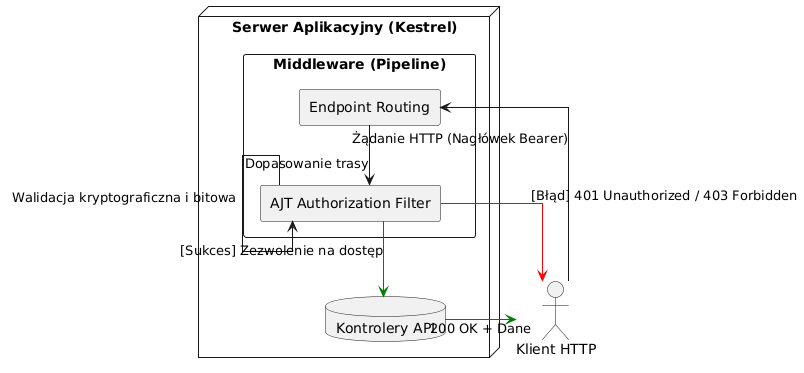
\includegraphics[width=0.8\textwidth]{png/aspnet_pipeline.png}
    \caption{Integracja filtru autoryzacyjnego z potokiem żądań ASP.NET Core}
    \label{fig:aspnet_pipeline}
\end{figure}

Zanim jednak filtr będzie mógł zwalidować żądanie (jak pokazano na schemacie), użytkownik musi najpierw wygenerować cyfrowe poświadczenie autentyczności, komunikując się z dedykowanym serwisem logowania.

\subsection{Proces logowania i generowania tokenów}

Serwis \texttt{LoginService} to główny punkt wejścia dla niezalogowanych użytkowników. Po poprawnej weryfikacji hasła system orkiestruje proces budowy i podpisywania poświadczeń. Użyto tu asynchronicznego dostępu do bazy danych, aby nie blokować głównego wątku serwera. Poniższy fragment ukazuje proces tworzenia zunifikowanego obiektu DTO (ang. \textit{Data Transfer Object}) zawierającego parę tokenów.

\begin{verbatim}
public async Task<CombinedToken?> Login(string login, string password)
{
    // ... walidacja użytkownika i skrótu hasła ...
    var userRoles = await userRoleRepo.GetUserRoles(user);
    
    var token = new Token
    {
        Id = Guid.NewGuid(),
        UserId = user.Id,
        Data = await _tokenDataService.GetCustomTokenData(user.Id),
        ExpirationDate = DateTime.Now.Add(_options.Value.TokenExpirationTime)
    };

    if (userRoles is not null)
        token.UserRoles = await _roleService.EncodeRoles(
            userRoles.Select(x => x.RoleCode).ToList());

    // ... wygenerowanie i zapis obiektu RefreshToken w bazie ...
    
    return new CombinedToken
    {
        Token = _hashingService.Hash(token),
        RefreshToken = _hashingService.Hash(refreshToken)
    };
}
\end{verbatim}

Analizując powyższy kod, należy zwrócić uwagę na wykorzystanie wstrzykniętych zależności. Serwis \texttt{\_roleService} przejmuje na siebie ciężar transformacji listy ról na format szesnastkowy (kompresja ról). Na samym końcu wywoływana jest metoda \texttt{Hash}, która zamienia struktury obiektowe C\# na docelowe ciągi znaków (ciągi zabezpieczone HMAC-SHA256).

\subsection{Implementacja odświeżania sesji i rotacji tokenów}

Zgodnie z wymaganiami architektonicznymi, czas życia wydanego tokenu (\texttt{TokenExpirationTime}) jest krótki. Proces podtrzymywania sesji znajduje się wewnątrz metody \texttt{Refresh}. Przyjmuje ona wygasający token odświeżający i implementuje proces rotacji kluczy w sposób bezpieczny.

W pierwszej kolejności następuje weryfikacja kryptograficzna. Odrzuca ona zapytania ze zmodyfikowanym ładunkiem od razu, oszczędzając zasoby serwera bazy danych. Następnie system weryfikuje ważność tokenu w warstwie persystencji. Kluczowym momentem w poniższym kodzie jest wywołanie metody \texttt{DeleteRefreshToken}. Zużycie starego tokenu natychmiast po jego weryfikacji, a przed wydaniem nowej pary poświadczeń, stanowi podstawowe zabezpieczenie przed atakami typu powtórzenia (ang. \textit{Replay Attack}).

\begin{verbatim}
public async Task<CombinedToken?> Refresh(string refreshTokenString)
{
    // 1. Szybka weryfikacja integralności kryptograficznej
    if (!_hashingService.VerifiyHash(refreshTokenString))
        return null;

    var payloadJson = _hashingService.DecodePayload(refreshTokenString);
    var oldRefreshToken = JsonConvert.DeserializeObject<RefreshToken>(payloadJson);

    using var scope = _scopeFactory.CreateScope();
    var refreshRepo = scope.ServiceProvider.GetRequiredService<IRefreshTokenRepo>();
    
    // 2. Weryfikacja obecności i ważności tokenu w relacyjnej bazie danych
    var dbToken = await refreshRepo.GetRefreshToken(oldRefreshToken.Id);
    if (dbToken is null || dbToken.ExpirationDate < DateTime.Now)
        return null;

    // 3. Rotacja - natychmiastowe usunięcie/zużycie starego tokenu
    await refreshRepo.DeleteRefreshToken(dbToken.Id);

    var userRepo = scope.ServiceProvider.GetRequiredService<IUserRepo>();
    var user = await userRepo.GetUserById(dbToken.UserId);

    // 4. Wygenerowanie nowej pary (Access Token + nowy Refresh Token)
    return await CreateCombinedTokenForUser(scope, user);
}
\end{verbatim}

\subsection{Dynamiczne rozszerzanie ładunku (Custom Payload)}

Aby stworzona biblioteka mogła funkcjonować jako uniwersalne narzędzie typu \textit{Plug and Play} w dowolnym projekcie, nie mogła ograniczać się wyłącznie do przechowywania ID użytkownika i ról. Zastosowano wzorzec strategii z wykorzystaniem delegatów \texttt{Func} zdefiniowanych w języku C\#. 

Poprzez konfigurację środowiskową, programista aplikacji nadrzędnej może wstrzyknąć funkcję zwrotną (ang. \textit{Callback}). Funkcja ta jest wywoływana dynamicznie podczas każdego procesu logowania. Daje ona dostęp do \texttt{IServiceProvider}, co pozwala odpytać inne moduły systemu (np. zewnętrzny serwis HR o numer departamentu pracownika) i "dokleić" ten niestandardowy obiekt do właściwości \texttt{Data} w tokenie.

\begin{verbatim}
// Delegat wywoływany wstrzyknięty podczas konfiguracji biblioteki
public void AddCustomTokenDataFunc(Func<Guid, IServiceProvider, Task<object>> func)
{
    _customTokenDataFunc = func;
}

// Użycie delegata wewnątrz usługi budującej ładunek tokenu
public async Task<object> GetCustomTokenData(Guid userId)
{
    if (_options.Value.CustomTokenDataFunc != null)
        return await _options.Value.CustomTokenDataFunc(userId, _serviceProvider);
        
    return null; // Zwróć null, jeśli deweloper nie rozszerzył modelu
}
\end{verbatim}

\clearpage

\subsection{Automatyzacja zarządzania rolami (Refleksja)}

Mechanizm operacji bitowych do weryfikacji ról jest wysoce zoptymalizowany, ale wymusza, by każda rola posiadała unikalny, sekwencyjny identyfikator numeryczny. Aby zdjąć z dewelopera obowiązek ręcznego uzupełniania bazy danych po dopisaniu nowej roli w kodzie, zaimplementowano tło asynchroniczne – \texttt{RoleBootstrapper}. 

Klasa ta implementuje interfejs \texttt{IHostedService}, co oznacza, że uruchamia się przed otwarciem głównych portów nasłuchujących serwera. Wykorzystując potężny mechanizm refleksji przestrzeni \texttt{System.Reflection}, algorytm ładuje do pamięci wszystkie skompilowane biblioteki (ang. \textit{Assemblies}), lokalizuje kontrolery i skanuje je pod kątem występowania atrybutów \texttt{[AllowRole]}.

\begin{verbatim}
protected override async Task ExecuteAsync(CancellationToken cancellationToken)
{
    // ... inicjalizacja dostępu do repozytorium przez IServiceProvider ...
    
    // Użycie refleksji do odnalezienia wszystkich kontrolerów API
    var controllers = AppDomain.CurrentDomain.GetAssemblies()
        .SelectMany(x => x.GetTypes())
        .Where(x => typeof(ControllerBase).IsAssignableFrom(x));

    var rolesFromAttributes = new HashSet<string>();

    foreach (var controller in controllers)
    {
        // Pobranie atrybutów z klas i metod bez ich uruchamiania
        var attributes = controller.GetCustomAttributes<AllowRoleAttribute>(true);
        // ... wyciągnięcie nazw ról z atrybutów i dodanie ich do zbioru (HashSet)
    }
    
    // ... porównanie zawartości zbioru ze stanem bazy danych.
    // Dopisanie brakujących ról wraz z wygenerowaniem sekwencyjnego numeru.
}
\end{verbatim}

Dzięki takiemu architektonicznemu podejściu system ról uczy się i adaptuje całkowicie samoczynnie (tzw. mechanizm \textit{Self-Discovery}).

\subsection{Implementacja kryptografii i ochrona Timing Attack}

Serwis \texttt{HashingService} realizuje logiczny proces powstawania skrótu HMAC. To właśnie w tym miejscu standardowy ciąg Base64 pozbawiany jest znaków kłopotliwych dla nawigacji HTTP.

Co niezwykle istotne, podczas implementacji weryfikacji podpisów w metodzie \texttt{VerifiyHash} zidentyfikowano potencjalne zagrożenie związane z atakami czasowymi (ang. \textit{Timing Attacks}). Standardowy operator porównania ciągów znaków (np. \texttt{==}) przerywa działanie natychmiast po napotkaniu pierwszej różnicy. Atakujący, analizując mikrosekundowe opóźnienia w odpowiedziach serwera przy przesyłaniu spreparowanych podpisów, mógłby krok po kroku odgadnąć cały skrót. Z tego powodu zaimplementowano stałoczasową weryfikację.

\begin{verbatim}
public bool VerifiyHash(string token)
{
    // ... podział tokenu na ładunek i podpis ...
    string expectedSignature = CreateSignature(unsignedToken, _options.Value.Secret);

    var signatureBytes = Encoding.UTF8.GetBytes(signature);
    var expectedBytes = Encoding.UTF8.GetBytes(expectedSignature);

    // Zabezpieczenie: Stałoczasowe porównanie zapobiegające Timing Attack
    return CryptographicOperations.FixedTimeEquals(signatureBytes, expectedBytes);
}

private static string CreateSignature(string unsignedToken, string secret)
{
    var keyBytes = Encoding.UTF8.GetBytes(secret);
    var messageBytes = Encoding.UTF8.GetBytes(unsignedToken);

    using var hmac = new HMACSHA256(keyBytes);
    var hash = hmac.ComputeHash(messageBytes);
    
    return Base64UrlEncode(hash); // Własna funkcja modyfikująca standardowy Base64
}
\end{verbatim}

\subsection{Filtr autoryzacyjny potoku HTTP}

Zwieńczeniem całego systemu jest przechwytywanie zapytań (zaprezentowane na schemacie \ref{fig:aspnet_pipeline}). Rdzeniem decyzyjnym jest klasa \texttt{AllowRoleFilter}, będąca implementacją \texttt{IAsyncAuthorizationFilter}.

Filtr sprawdza warunki bezpieczeństwa. Jeśli algorytm \texttt{VerifiyHash} zawiedzie (zmodyfikowany ładunek lub inna manipulacja), zwracany jest kod statusu \texttt{401 Unauthorized} (brak uwierzytelnienia). Z kolei jeśli użytkownik ma poprawny token, ale algorytm bitowy \texttt{DecodeRoles} wykaże brak wymaganej roli dla danego zasobu, zwracany jest kod statusu \texttt{403 Forbidden} (brak autoryzacji do konkretnego zasobu), co stanowi implementacyjną realizację zasad rozdzielności tych pojęć.

\begin{verbatim}
public async Task OnAuthorizationAsync(AuthorizationFilterContext context)
{
    // ... sprawdzenie i wyciągnięcie nagłówka Bearer Token ...
    
    if (!_hashingService.VerifiyHash(token))
    {
        context.HttpContext.Response.StatusCode = 401; // Unauthorized
        return;
    }

    // Dekodowanie identyfikatorów z formatu szesnastkowego z powrotem na nazwy
    var userRoles = await _roleService.DecodeRoles(tokenObject.UserRoles);
    
    // Weryfikacja zbioru uprawnień bitowych
    foreach (var requiredRole in _roles)
    {
        if (userRoles.Contains(requiredRole))
            return; // Zezwól na dostęp - przekaż żądanie do kontrolera
    }
    
    context.HttpContext.Response.StatusCode = 403; // Forbidden
}
\end{verbatim}

\section{Analiza bezpieczeństwa i testowanie}

Istotnym etapem cyklu życia oprogramowania nastawionego na autoryzację jest empiryczna walidacja jego podatności. Rozdział ten skupia się na ocenie zaprojektowanego systemu przez pryzmat uznanego w branży standardu OWASP Top 10, szczegółowym omówieniu zautomatyzowanych testów bezpieczeństwa oraz nakreśleniu perspektyw dalszego rozwoju w aspektach, które wykraczały poza ramy obecnej iteracji prac.

\subsection{Zgodność ze standardem OWASP Top 10}

OWASP Top 10 to najpopularniejszy, globalny dokument uświadamiający zagrożenia bezpieczeństwa aplikacji internetowych. Biblioteka autoryzacyjna została zaprojektowana w oparciu o ideę \textit{Security by Design}, co ogranicza ekspozycję na najczęstsze z klasyfikowanych podatności:

\begin{itemize}
    \item \textbf{Broken Access Control (Naruszenie kontroli dostępu):} W modelu Zero Trust każda metoda API pozbawiona weryfikacji stanowi ryzyko eskalacji uprawnień. System eliminuje to zagrożenie poprzez sztywne wpięcie logiki decyzyjnej do potoku wykonawczego. Co więcej, rygorystyczne operacje oparte na matematycznych maskach bitowych nie pozwalają na manipulację ciągami tekstowymi ról (np. próbę nadpisania parametru \texttt{role="admin"}) przez nieuprzywilejowanych użytkowników.
    \item \textbf{Cryptographic Failures (Błędy kryptograficzne):} Poufność haseł została zapewniona poprzez wykorzystanie silnych skrótów kryptograficznych wraz z mechanizmem solenia (ang. \textit{Salting}), co całkowicie uniemożliwia odzyskanie haseł tekstowych nawet w przypadku fizycznego wycieku bazy danych. Integralność samego tokenu opiera się o sprawdzony standard z rodziny SHA-256 i unikalny sekretny klucz.
    \item \textbf{Injection (Wstrzykiwanie kodu):} System wykorzystuje mapowanie obiektowo-relacyjne Entity Framework Core, które pod warstwą abstrakcji zawsze używa zapytań parametryzowanych. Architektura ta całkowicie neutralizuje zagrożenia związane z SQL Injection, uniemożliwiając wykonanie preparowanych zapytań modyfikujących strukturę relacyjną.
    \item \textbf{Identification and Authentication Failures (Błędy identyfikacji):} Implementacja rotacji tokenów odświeżających (opisana w poprzednich rozdziałach) oraz natychmiastowe usuwanie zużytych poświadczeń skutecznie chroni aplikację przed atakami typu \textit{Session Fixation} oraz \textit{Replay Attack} (atak polegający na przechwyceniu i ponownym wykorzystaniu starego żądania uwierzytelniającego).
    \item \textbf{Security Misconfiguration (Błędy konfiguracji zabezpieczeń):} Biblioteka wymusza na programiście dostarczenie klucza szyfrującego z poziomu konfiguracji zewnętrznej (poprzez wstrzyknięcie obiektu \texttt{AJTOptions}). Wymusza to odseparowanie kluczy od kodu źródłowego, chroniąc przed ich przypadkowym ujawnieniem w repozytoriach publicznych (np. GitHub).
\end{itemize}

\subsection{Zautomatyzowane testy bezpieczeństwa (Security Unit Testing)}

Najbardziej newralgicznym elementem zaprojektowanej architektury jest weryfikacja kryptograficzna podpisu, od której zależy ostateczne zaufanie do zawartości tokenu. Błąd na tym etapie skutkowałby całkowitym przełamaniem systemu autoryzacji. Aby udowodnić nienaruszalność mechanizmu, kod poddano rygorystycznym testom jednostkowym z wykorzystaniem frameworka \textit{xUnit} oraz biblioteki \textit{FluentAssertions}.

\textbf{Test 1: Odporność na wstrzykiwanie uprawnień (Tampering)}

Pierwszy, najważniejszy scenariusz weryfikuje zjawisko wstrzykiwania uprawnień. Atakujący, znając format Base64Url, mógłby zdekodować pierwszą część tokenu, zmienić swoje uprawnienia (np. z "00" na "01" reprezentujące wyższą rolę), a następnie zakodować ją ponownie, pozostawiając stary podpis. Test dowodzi, że weryfikator natychmiast odrzuci tak zmodyfikowany ładunek.

\begin{verbatim}
[Fact]
public void VerifyHash_GivenTamperedToken_ShouldReturnFalse()
{
    // Arrange: Wygenerowanie poprawnego tokenu z najniższymi uprawnieniami
    var token = new Token { Id = Guid.NewGuid(), UserRoles = "00" };
    var hashedToken = _sut.Hash(token);
    
    // Act: Symulacja ataku poprzez modyfikację zawartości ładunku
    // bez przeliczania algorytmu HMAC (brak znajomości klucza tajnego).
    var tamperedToken = hashedToken.Replace("00", "01");

    var isValid = _sut.VerifiyHash(tamperedToken);

    // Assert: Weryfikacja musi jednoznacznie odrzucić token
    isValid.Should().BeFalse();
}
\end{verbatim}

\textbf{Test 2: Izolacja kryptograficzna kluczy serwerowych}

Kolejny scenariusz bezpieczeństwa zakłada próbę użycia tokenu podpisanego przez inny system (lub wygenerowanego przed rotacją głównego klucza serwera). Token poprawnie sformatowany, ale posiadający podpis wygenerowany innym kluczem tajnym, musi zostać uznany za nieautoryzowany. Zapobiega to wykorzystaniu fałszywych serwerów tożsamości do generowania tokenów dostępowych.

\begin{verbatim}
[Fact]
public void VerifyHash_SignedWithDifferentKey_ShouldReturnFalse()
{
    // Arrange: Generowanie tokenu przez Serwer A (Atakujący)
    var originalOptions = Options.Create(new AJTOptions { Secret = "Secret_A" });
    var attackerSut = new HashingService(originalOptions);
    var forgedToken = attackerSut.Hash(new Token { Id = Guid.NewGuid() });

    // Instancja głównego Serwera B z prawidłowym kluczem
    var validOptions = Options.Create(new AJTOptions { Secret = "Secret_B" });
    var validSut = new HashingService(validOptions);

    // Act: Próba autoryzacji fałszywym tokenem na właściwym serwerze
    var isValid = validSut.VerifiyHash(forgedToken);

    // Assert: Token z obcym podpisem zostaje odrzucony
    isValid.Should().BeFalse();
}
\end{verbatim}

\textbf{Test 3: Odporność na uszkodzone struktury danych (Malformed Input)}

Ataki polegające na przesyłaniu uszkodzonych ciągów znaków (np. całkowitym usunięciu podpisu lub zaburzeniu separatorów) często prowadzą do wywoływania nieobsłużonych wyjątków serwera (ang. \textit{Unhandled Exceptions}), co może być wektorem ataków typu DoS (ang. \textit{Denial of Service}). Test wykorzystuje parametryzację (\texttt{[Theory]}), aby upewnić się, że funkcja weryfikująca "kulturalnie" odrzuca takie dane bez awarii aplikacji.

\begin{verbatim}
[Theory]
[InlineData("TylkoJedenSegmentBezKropki")]
[InlineData("Segment1.Segment2.Segment3.ZaDuzoKropek")]
[InlineData(".TylkoPodpis")]
[InlineData("TylkoLadunek.")]
[InlineData("")]
public void VerifyHash_GivenMalformedFormat_ShouldReturnFalse(string malformedInput)
{
    // Act
    var isValid = _sut.VerifiyHash(malformedInput);

    // Assert: Wszystkie niepoprawne formaty dają wynik negatywny
    // Serwer nie ulega awarii (brak wyjątków NullReferenceException itp.)
    isValid.Should().BeFalse();
}
\end{verbatim}

\subsection{Ograniczenia systemu i obszary dalszego rozwoju}

Świadomość ograniczeń wyprodukowanego kodu stanowi miarę inżynierskiej dojrzałości projektu. Choć system spełnia założenia optymalizacyjne w zakresie objętości danych, jego implementacja pozostawia pole do rozbudowy w przyszłych iteracjach badawczych. 

\textbf{Czarna lista tokenów (Blacklisting):} W pierwszej kolejności nie zaimplementowano tzw. czarnej listy tokenów. Ponieważ serwer z założenia nie odpytuje bazy danych przy walidacji \textit{Access Tokenu}, w przypadku jawnego wylogowania lub przejęcia poświadczeń z przeglądarki użytkownika, token pozostaje ważny aż do czasu naturalnego wygaśnięcia. Wdrożenie zewnętrznej, błyskawicznej bazy pamięciowej (np. Redis), która przechowywałaby identyfikatory unieważnionych tokenów z przypisanym czasem życia (ang. \textit{Time-To-Live}) dopasowanym do ich wygaśnięcia, skutecznie załatałoby tę lukę bez drastycznego spadku wydajności.

\textbf{Kryptografia asymetryczna:} Brak implementacji kryptografii asymetrycznej ogranicza wdrożenie systemu do prostszych środowisk. Obecny symetryczny algorytm HMAC-SHA256 sprawdza się w przypadku monolitycznego API, lecz w wysoce rozproszonej architekturze wymagane byłoby współdzielenie tego samego klucza tajnego między wszystkimi jednostkami infrastruktury, co stanowi znaczne ryzyko kradzieży. Implementacja wsparcia dla algorytmów z rodziny RSA lub ECDSA (gdzie centralny serwer autoryzacyjny używa klucza prywatnego do podpisu, a mikroserwisy używają ogólnodostępnego klucza publicznego do weryfikacji) stanowiłaby krytyczne rozszerzenie możliwości biblioteki.

\textbf{Ochrona przed atakami Brute-Force:} Autorski system nie posiada wbudowanych mechanizmów limitowania zapytań sieciowych. Konsekwencją tego jest teoretyczna podatność punktu końcowego realizującego funkcję logowania na ataki siłowe (ang. \textit{Brute-Force}) lub ataki słownikowe (ang. \textit{Credential Stuffing}). W przyszłości biblioteka powinna zostać zintegrowana z natywnym modułem \textit{ASP.NET Core Rate Limiting}, aby automatycznie blokować numery IP generujące anomalną liczbę błędnych prób uwierzytelnienia.

\clearpage

\section{Podsumowanie}

Głównym celem niniejszej pracy inżynierskiej było zaprojektowanie i zaimplementowanie autorskiego, zoptymalizowanego systemu uwierzytelniania i autoryzacji dla aplikacji opartych o środowisko ASP.NET Core. Poprzez analizę powszechnie stosowanych technologii sieciowych oraz wymagań współczesnych norm bezpieczeństwa, udowodniono skuteczność paradygmatu \textit{Zero Trust} wspomaganego szybkimi, bezstanowymi tokenami.

Opracowana biblioteka pomyślnie rozwiązuje problem strukturalnego narzutu przesyłowych danych obecnego w popularnym standardzie JWT. Eliminacja nieużywanych metadanych oraz innowacyjne, oparte na konwersji bitowej podejście do interpretowania złożonych struktur ról użytkowników zaowocowały miniaturyzacją autoryzacyjnych żądań sieciowych. Wykorzystanie warstwy abstrakcji programistycznej, zgodnej z wzorcami wstrzykiwania zależności, umożliwiło zamknięcie całej złożoności w zgrabnym, hermetycznym module o minimalnym progu wejścia (ang. \textit{low entry barrier}) dla przyszłych programistów. 

Przeprowadzona analiza testowa w oparciu o globalne wytyczne OWASP potwierdziła, że kompresja algorytmów nie wpłynęła na obniżenie parametrów zabezpieczeń kryptograficznych. Choć uwypuklono obszary do potencjalnej kontynuacji badań technologicznych – takie jak implementacja natywnych rozwiązań pamięci podręcznej dla autoryzacji czy kluczy asymetrycznych – wykreowane rozwiązanie spełnia zadane wymogi inżynierskie i stanowi w pełni funkcjonalną alternatywę autoryzacyjną dla systemów o klasycznym i mikroserwisowym profilu architektonicznym.

\end{document}